\chapter{Enclosure Design}
To complete the device design, a custom enclosure was created to house both the readout PCB and the user board. The enclosure is designed to protect the sensitive electronics while ensuring adequate airflow for thermal management. It consists of three main components: 

\begin{itemize}
    \item \textbf{Bottom Shell}: This part includes holes for the reset button, boot button, and LED indicator.
    \item \textbf{Sleeve}: This section features cutouts for all the SMA connectors and the USB port.
    \item \textbf{Top Shell}: This piece fully encloses the readout PCB.
\end{itemize}

Holes for metal heat inserts are located in the corners. Once the inserts are in place, the three parts are secured together using four M2 screws. The user board can be easily disconnected from the readout PCB. If needed, it can also be fixed in place using M2 screws. The placement of the inserts and screws is depicted in Figure \ref{fig:readout_inserts}.

\FloatBarrier
\begin{figure}[htp!]
    \centering
    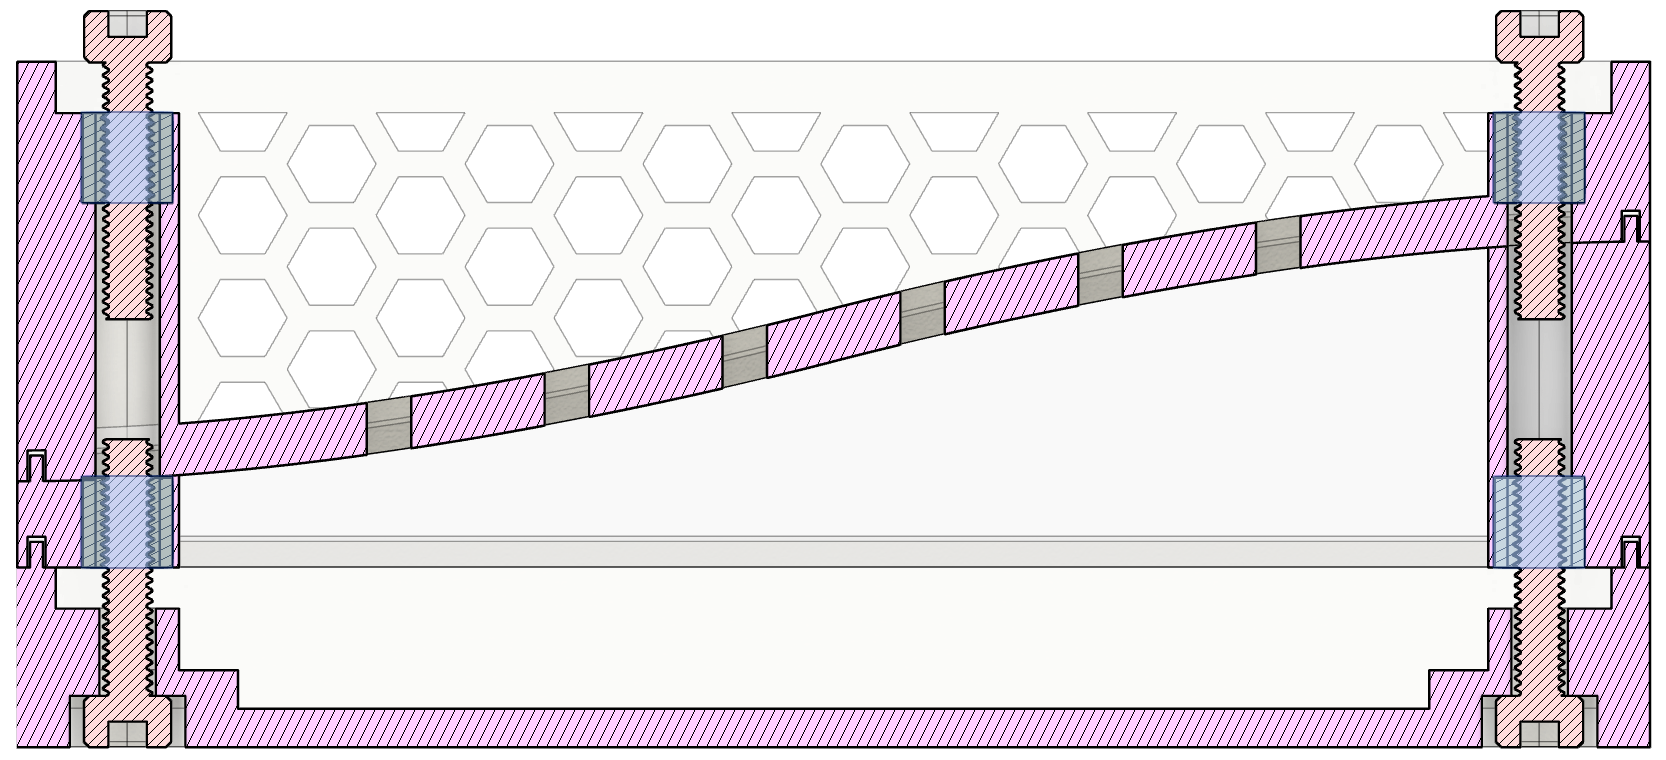
\includegraphics[height=4cm]{insert.png}
    \caption{Metal insert placement}
    \label{fig:readout_inserts}
\end{figure}
\FloatBarrier

The enclosure was designed to be 3D printed using a standard \emph{FDM} printer. The top shell and sleeve can either be printed separately and glued together, or they can be printed as a one piece on multi material printer. The design process was carried out in Fusion 360. Renders of the enclosure are shown below.

\FloatBarrier
\begin{figure}[htp!]
    \centering
    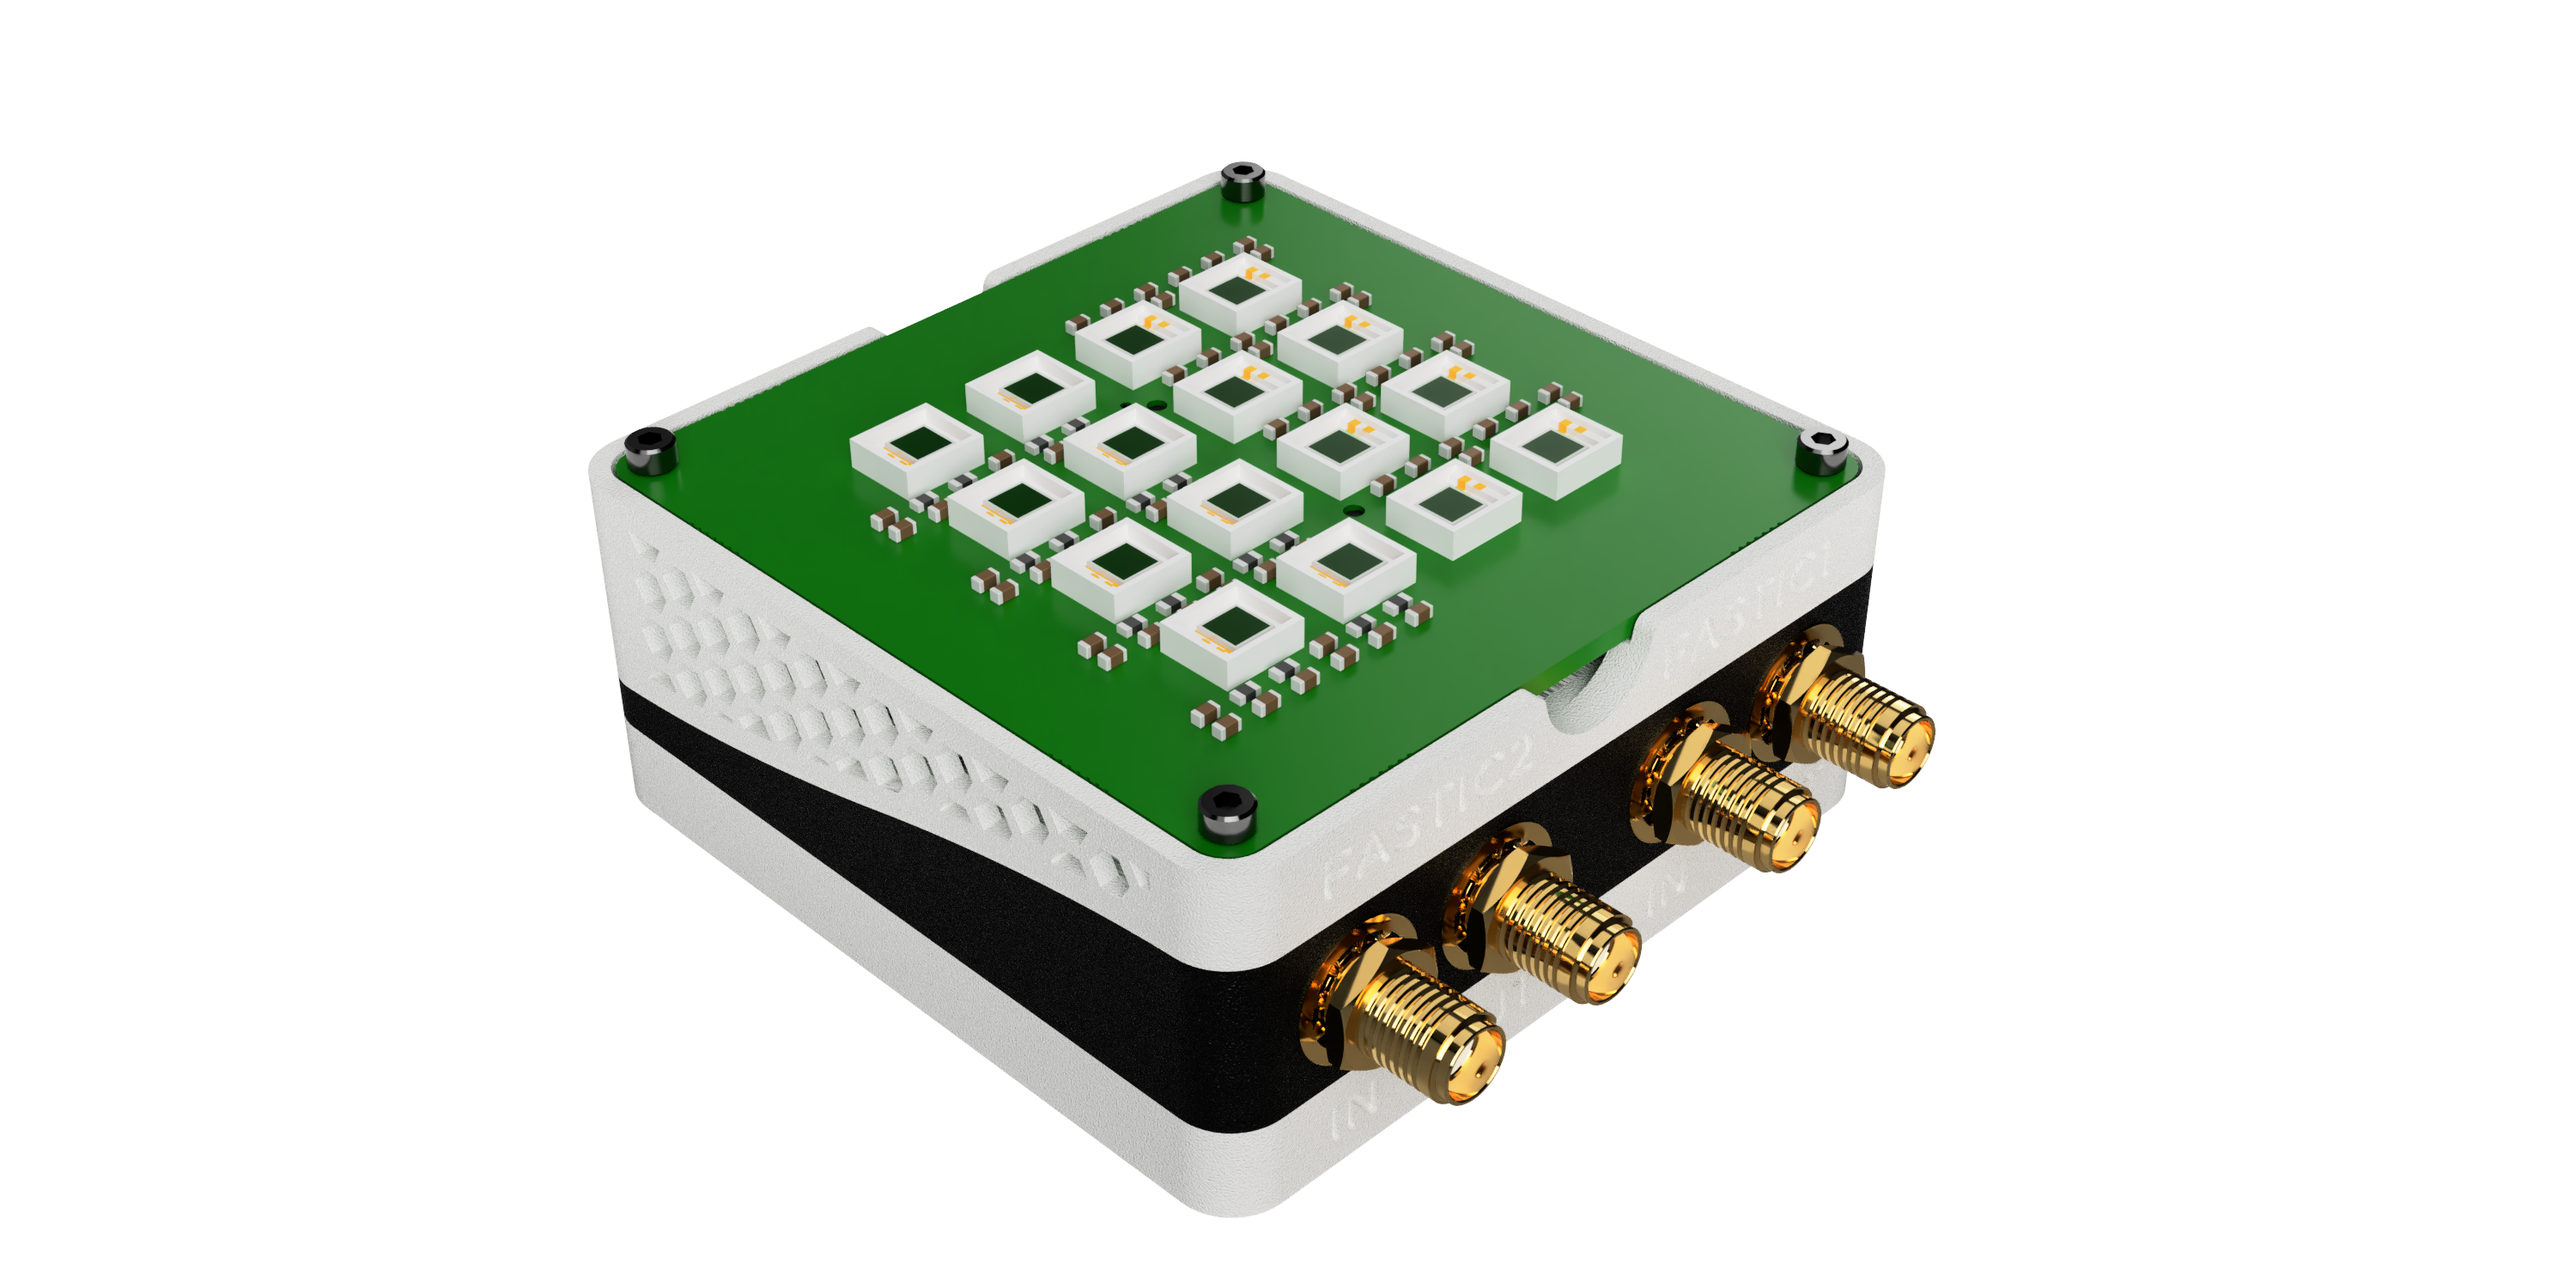
\includegraphics[height=8cm,trim={11cm 0 11cm 0},clip]{mech_preview.png}
    \caption{3D Preview of the Readout PCB Enclosure}
    \label{fig:readout_3d_preview}
\end{figure}
\FloatBarrier

\FloatBarrier
\begin{figure}[htp!]
    \centering
    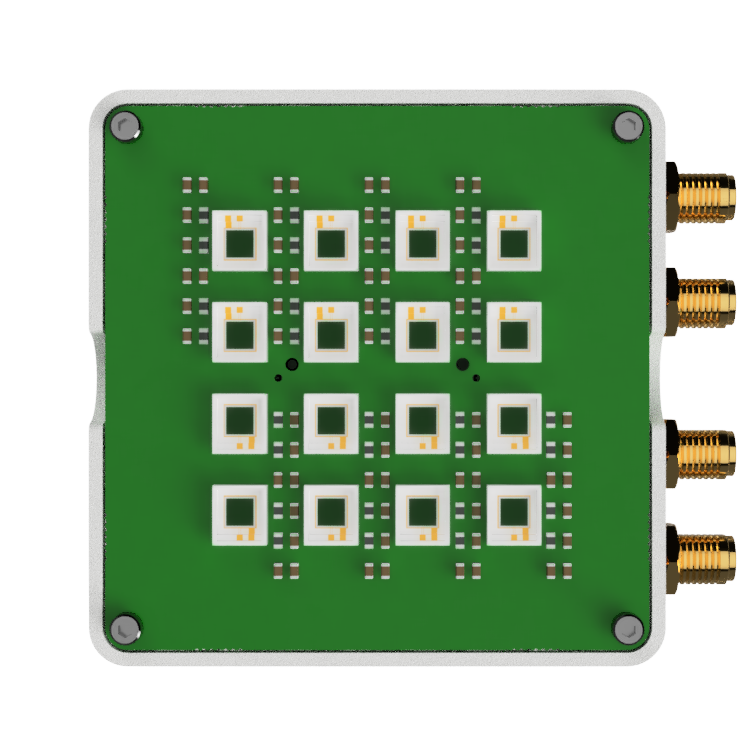
\includegraphics[height=6cm]{mech_top.png}
    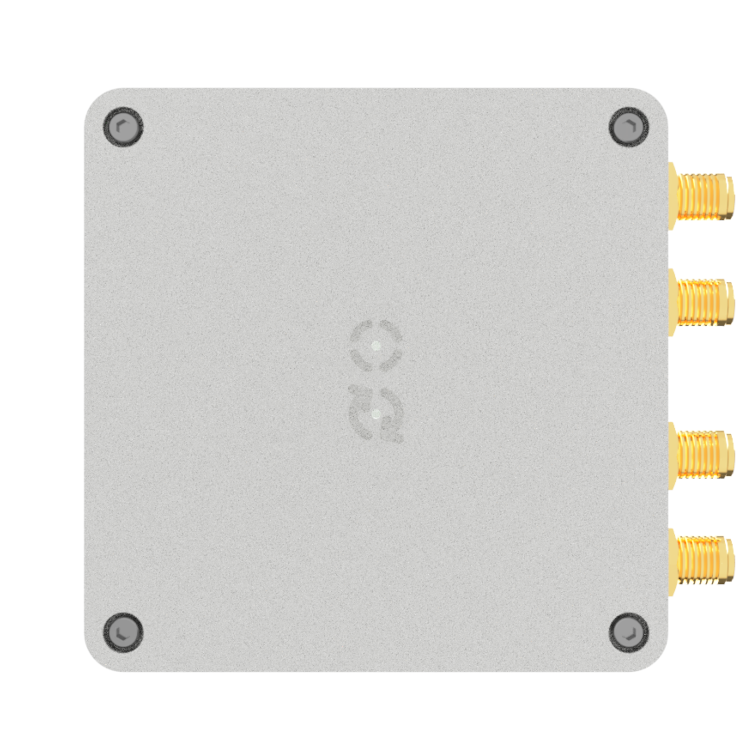
\includegraphics[height=6cm]{mech_bottom.png}
    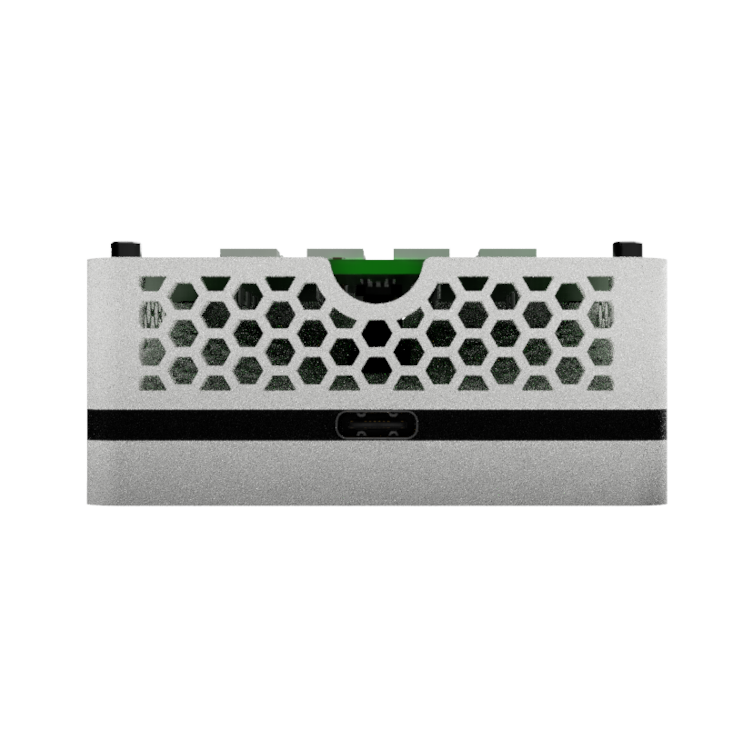
\includegraphics[height=6cm]{mech_front.png}
    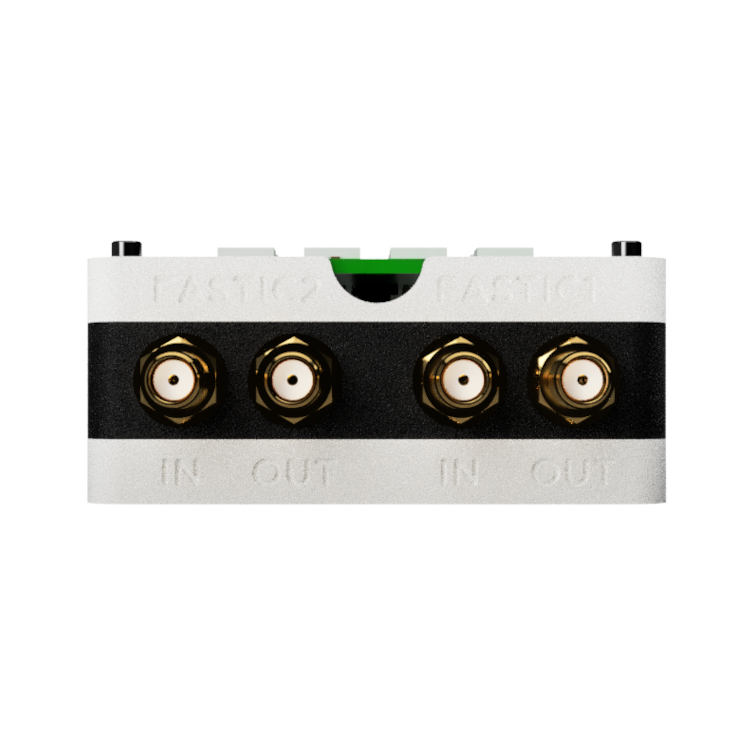
\includegraphics[height=6cm]{mech_rear.png}
    \caption{Top, Bottom, Front, and Rear Views of the Enclosure}
    \label{fig:readout_3d_views}
\end{figure}
\FloatBarrier
